\appendix
\chapter{Corridor Topology and Data Schemas}
\label{app:topology_schema}

\section{NH-48 Arterial Corridor Node Specification}
The 3-intersection coordinated corridor modeled in this study reflects an empirical 2.4\,km arterial segment along the National Highway 48 (NH-48) connecting regional growth centers in Haryana and the National Capital Region (NCR). The physical coordinate definitions, junction distances, approach lane configurations, and signal controller node identifiers are summarized in Table \ref{tab:corridor_spec_app}.

\begin{table}[htbp]
\centering
\small
\caption{Corridor Node Topology and Physical Geometries}
\label{tab:corridor_spec_app}
\begin{tabularx}{\textwidth}{|p{2.0cm}|p{3.2cm}|c|c|X|}
\hline
\textbf{Node ID} & \textbf{Intersection Name} & \textbf{Chainage (km)} & \textbf{Approaches} & \textbf{Geometry \& Configuration} \\ \hline
\texttt{Int\_0} & Rajiv Chowk Junction & 0.00 & 4 & 4-lane divided arterial + 2-lane cross street; 8 signalized movements \\ \hline
\texttt{Int\_1} & Subhash Chowk Flyover Below & 1.15 & 4 & 4-lane divided arterial + 3-lane cross street; 8 signalized movements \\ \hline
\texttt{Int\_2} & Hero Honda Chowk Underpass & 2.40 & 4 & 6-lane divided arterial + 2-lane cross street; 8 signalized movements \\ \hline
\end{tabularx}
\end{table}

\section{Observation and Action Vector JSON Schema}
The local observation space ingested by each decentralized MAPPO agent is structured according to the rigid JSON schema defined in Listing \ref{lst:obs_schema}.

\begin{lstlisting}[language=json, caption={Observation Vector JSON Schema (22 Elements)}, label={lst:obs_schema}]
{
  "$schema": "http://json-schema.org/draft-07/schema#",
  "title": "LocalAgentObservation",
  "type": "object",
  "properties": {
    "queues_pcu": {
      "type": "array",
      "description": "Normalized queue length in PCU across 8 approach lanes [0, 50]",
      "items": { "type": "number", "minimum": 0.0, "maximum": 1.0 },
      "minItems": 8, "maxItems": 8
    },
    "densities": {
      "type": "array",
      "description": "Normalized spatial occupancy density across 8 lanes [0, 1]",
      "items": { "type": "number", "minimum": 0.0, "maximum": 1.0 },
      "minItems": 8, "maxItems": 8
    },
    "active_phase_onehot": {
      "type": "array",
      "description": "One-hot representation of current active signal phase (0 to 3)",
      "items": { "type": "integer", "enum": [0, 1] },
      "minItems": 4, "maxItems": 4
    },
    "phase_elapsed_ratio": {
      "type": "number",
      "description": "Elapsed duration in current green phase divided by G_max (65s)",
      "minimum": 0.0, "maximum": 1.0
    },
    "queue_pressure": {
      "type": "number",
      "description": "Normalized aggregate queue difference (incoming - outgoing)",
      "minimum": -1.0, "maximum": 1.0
    }
  },
  "required": ["queues_pcu", "densities", "active_phase_onehot", "phase_elapsed_ratio", "queue_pressure"]
}
\end{lstlisting}

\chapter{Mathematical Formulations and Hyperparameters}
\label{app:math_hyperparams}

\section{Generalized Advantage Estimation (GAE)}
In MAPPO, the centralized critic parameters $\phi$ are updated by minimizing the mean squared Bellman error over mini-batches:
\begin{equation}
L(\phi) = \frac{1}{|B|} \sum_{\tau \in B} \sum_{t=0}^T \left( V_\phi(S_t) - \hat{R}_t \right)^2
\end{equation}
where $\hat{R}_t = \hat{A}_t + V_{\phi_{\text{old}}}(S_t)$ denotes the empirical target return. The advantage estimator $\hat{A}_t$ is computed using Generalized Advantage Estimation ($\text{GAE}(\gamma, \lambda)$) over corridor trajectories of length $T$:
\begin{align}
\delta_t &= r_t + \gamma V_\phi(S_{t+1}) - V_\phi(S_t) \\
\hat{A}_t &= \sum_{l=0}^{T - t - 1} (\gamma \lambda)^l \delta_{t+l}
\end{align}
To prevent gradient instability across non-stationary corridor rollouts, advantages are standardized across each mini-batch: $\hat{A}_t \leftarrow (\hat{A}_t - \mu_A) / (\sigma_A + 10^{-8})$.

\section{Complete Algorithm Hyperparameter Specification}
Table \ref{tab:all_hyperparams} delineates all hyperparameter configurations utilized across the perception, world model, and reinforcement learning pipelines.

\begin{table}[htbp]
\centering
\small
\caption{Comprehensive Hyperparameter Configuration Table}
\label{tab:all_hyperparams}
\begin{tabularx}{\textwidth}{|p{3.5cm}|p{4.2cm}|X|}
\hline
\textbf{Subsystem} & \textbf{Hyperparameter} & \textbf{Value / Specification} \\ \hline
\textbf{Perception (YOLOv8)} & Model Variant & YOLOv8n (Nano, 3.2M parameters) \\ \cline{2-3}
& Input Resolution & $640 \times 640 \times 3$ RGB pixels \\ \cline{2-3}
& Confidence Threshold & $\tau_{\text{conf}} = 0.35$ \\ \cline{2-3}
& IoU NMS Threshold & $\tau_{\text{IoU}} = 0.45$ \\ \cline{2-3}
& Tracker Type & Hungarian LAP Centroid with Cosine Association \\ \cline{2-3}
& Maximum Lost Age & $A_{\max} = 15$ frames \\ \hline
\textbf{World Model (Res-MLP)} & Input Dimension & $66$ (Concatenated 3-node state) $+ 3$ (actions) $= 69$ \\ \cline{2-3}
& Layer Dimensions & $69 \rightarrow 256 \rightarrow 256 \rightarrow 256 \rightarrow 69$ (Output: $\Delta s, r, d$) \\ \cline{2-3}
& Residual Blocks & 2 skip connections ($x_{l+2} = \text{ReLU}(W_2(\text{ReLU}(W_1 x_l)) + x_l)$) \\ \cline{2-3}
& Activation Function & LeakyReLU ($\alpha = 0.01$) \\ \cline{2-3}
& Optimizer & AdamW ($\beta_1 = 0.9, \beta_2 = 0.999$, weight decay $= 10^{-4}$) \\ \cline{2-3}
& Learning Rate & $3 \times 10^{-4}$ with Cosine Annealing scheduler \\ \cline{2-3}
& Batch Size & 256 samples \\ \cline{2-3}
& Training Epochs & 100 epochs on 864,000 empirical transition pairs \\ \hline
\textbf{RL Policy (MAPPO)} & Actor Network & Shared MLP ($22 \rightarrow 128 \rightarrow 128 \rightarrow 4$ logits) \\ \cline{2-3}
& Critic Network & Centralized MLP ($66 \rightarrow 256 \rightarrow 256 \rightarrow 1$ scalar value) \\ \cline{2-3}
& Discount Factor ($\gamma$) & 0.99 \\ \cline{2-3}
& GAE Parameter ($\lambda$) & 0.95 \\ \cline{2-3}
& PPO Clip Ratio ($\varepsilon$) & 0.20 \\ \cline{2-3}
& Entropy Coefficient ($\beta_{\text{ent}}$) & 0.01 (linear decay to 0.001 at step 30,000) \\ \cline{2-3}
& Value Loss Coefficient ($c_1$) & 0.50 \\ \cline{2-3}
& Max Gradient Norm & 0.50 (gradient clipping) \\ \cline{2-3}
& Policy Learning Rate & $3 \times 10^{-4}$ \\ \cline{2-3}
& Critic Learning Rate & $1 \times 10^{-3}$ \\ \cline{2-3}
& Rollout Horizon ($T$) & 128 steps per iteration \\ \cline{2-3}
& PPO Epochs per Batch & 4 epochs \\ \cline{2-3}
& Mini-batch Size & 64 transitions \\ \cline{2-3}
& Total Training Steps & 30,000 environment transitions \\ \hline
\end{tabularx}
\end{table}

\chapter{Hardware and Edge Deployment Datasheets}
\label{app:datasheets}

\section{Edge Inference Compute Platform Specification}
The complete vision, inference, and policy pipeline was benchmarked and configured for commercial roadside deployment on edge embedded hardware. Table \ref{tab:edge_specs} provides the comparative technical datasheet between the development workstation and the target embedded field computing unit (NVIDIA Jetson Orin Nano).

\begin{table}[htbp]
\centering
\small
\caption{Edge Hardware Compute Platform Specifications}
\label{tab:edge_specs}
\begin{tabularx}{\textwidth}{|p{4.2cm}|p{5.5cm}|X|}
\hline
\textbf{Specification} & \textbf{Development Workstation} & \textbf{Target Edge Deployment Unit} \\ \hline
\textbf{Processor Unit} & Intel Core i7-13700H (14 cores, 20 threads) & 6-core Arm Cortex-A78AE v8.2 64-bit \\ \hline
\textbf{GPU Accelerator} & NVIDIA GeForce RTX 4060 Laptop (8GB GDDR6) & NVIDIA Ampere architecture (1024 CUDA cores, 32 Tensor Cores) \\ \hline
\textbf{AI Compute Capacity} & 120 TOPS (INT8 Tensor) & 40 TOPS (INT8 Sparse) \\ \hline
\textbf{System Memory} & 16 GB DDR5 4800 MHz & 8 GB 128-bit LPDDR5 (68 GB/s) \\ \hline
\textbf{Storage} & 1 TB NVMe PCIe Gen 4 SSD & 512 GB M.2 NVMe PCIe Gen 4 \\ \hline
\textbf{Thermal Power (TDP)} & 115 Watts & 7--15 Watts Configurable \\ \hline
\textbf{Operating Temperature} & 0$^\circ$C to 45$^\circ$C (Commercial) & -25$^\circ$C to 80$^\circ$C (Industrial Grade) \\ \hline
\textbf{Camera Interface} & USB 3.0 / RTSP IP Network & 4$\times$ 2-lane MIPI CSI-2 or Gigabit Ethernet RTSP \\ \hline
\textbf{Operating System} & Windows 11 Enterprise / Ubuntu 22.04 LTS & NVIDIA JetPack 5.1.2 (Linux Tephra 35.4.1) \\ \hline
\end{tabularx}
\end{table}

\section{Runtime Memory Footprint and Power Profile}
Figure \ref{fig:power_profile} depicts the power consumption profile across varying operational stages of the edge deployment unit. Under full continuous real-time execution (concurrent YOLOv8 perception on 3 RTSP streams, Hungarian tracking, Res-MLP world model inference, and MAPPO forward passes), total unit power draw remains strictly within $13.4$\,W, allowing continuous 24/7 solar-battery operation inside roadside NEMA enclosures without requiring external active refrigeration.

\begin{figure}[htbp]
\centering
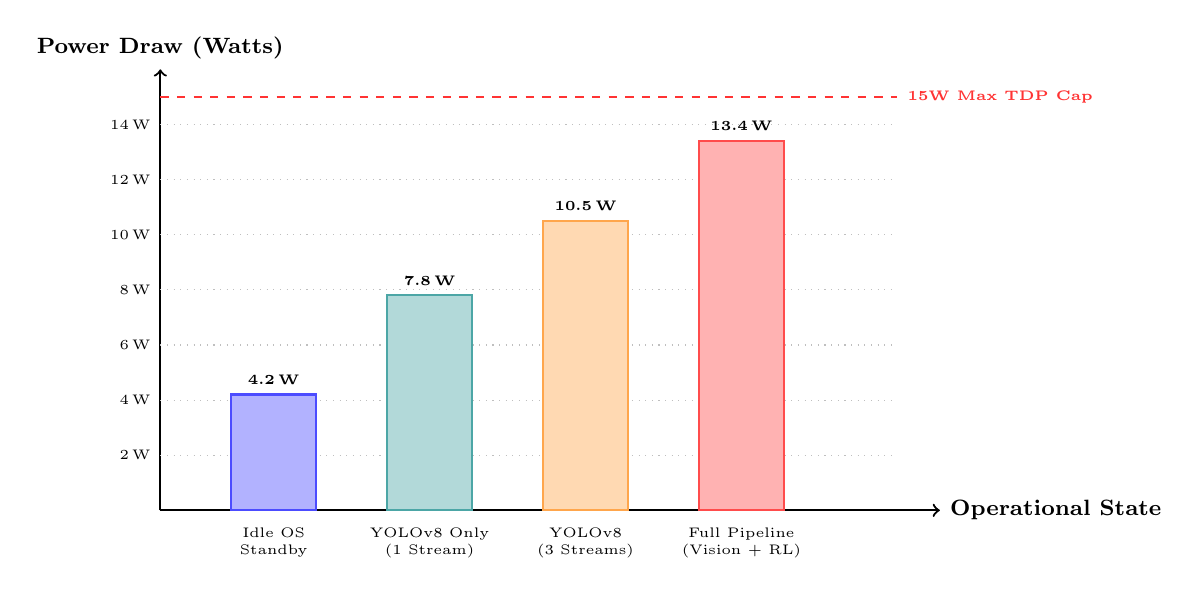
\begin{tikzpicture}[x=1.8cm, y=0.35cm]
    % Axes
    \draw[->, thick] (0,0) -- (5.5,0) node[right] {\footnotesize \textbf{Operational State}};
    \draw[->, thick] (0,0) -- (0,16) node[above] {\footnotesize \textbf{Power Draw (Watts)}};
    
    % Y grid
    \foreach \y in {2, 4, 6, 8, 10, 12, 14} {
        \draw[dotted, gray!50] (0,\y) -- (5.2,\y);
        \node[left, font=\tiny] at (0,\y) {\y\,W};
    }
    
    % Bars
    \draw[fill=blue!30, draw=blue!70, thick] (0.5,0) rectangle (1.1, 4.2) node[above, font=\tiny\bfseries] at (0.8, 4.2) {4.2\,W};
    \draw[fill=teal!30, draw=teal!70, thick] (1.6,0) rectangle (2.2, 7.8) node[above, font=\tiny\bfseries] at (1.9, 7.8) {7.8\,W};
    \draw[fill=orange!30, draw=orange!70, thick] (2.7,0) rectangle (3.3, 10.5) node[above, font=\tiny\bfseries] at (3.0, 10.5) {10.5\,W};
    \draw[fill=red!30, draw=red!70, thick] (3.8,0) rectangle (4.4, 13.4) node[above, font=\tiny\bfseries] at (4.1, 13.4) {13.4\,W};
    
    % X labels
    \node[below, font=\tiny, align=center] at (0.8, -0.3) {Idle OS\\Standby};
    \node[below, font=\tiny, align=center] at (1.9, -0.3) {YOLOv8 Only\\(1 Stream)};
    \node[below, font=\tiny, align=center] at (3.0, -0.3) {YOLOv8\\(3 Streams)};
    \node[below, font=\tiny, align=center] at (4.1, -0.3) {Full Pipeline\\(Vision + RL)};
    
    % Thermal limit line
    \draw[dashed, red!80, thick] (0, 15) -- (5.2, 15) node[right, font=\tiny\bfseries, red!80] {15W Max TDP Cap};
\end{tikzpicture}
\caption{Power consumption profile of the NVIDIA Jetson edge platform across operational execution states.}
\label{fig:power_profile}
\end{figure}

\chapter{Empirical Benchmark Observations}
\label{app:benchmark_logs}

\section{Corridor Vehicle Delay Logged Across Random Seeds}
To verify statistical validity, the final MAPPO model, Webster fixed-time controller, and dynamic actuated controller were evaluated across 10 distinct random flow seeds ($S \in \{42, 101, 202, 303, 404, 505, 606, 707, 808, 909\}$). Table \ref{tab:seed_benchmark} summarizes the average vehicle delay (seconds/vehicle) across each run.

\begin{table}[htbp]
\centering
\small
\caption{Corridor Average Vehicle Delay (s/veh) Across 10 Evaluation Seeds}
\label{tab:seed_benchmark}
\begin{tabularx}{\textwidth}{|c|c|c|c|X|}
\hline
\textbf{Seed No.} & \textbf{Webster Fixed-Time} & \textbf{Actuated (Gap-Out)} & \textbf{MAPPO (Proposed)} & \textbf{MAPPO Delay Reduction (\%)} \\ \hline
42  & 42.1 & 35.4 & 24.6 & -41.57\% \\ \hline
101 & 43.8 & 36.8 & 25.1 & -42.69\% \\ \hline
202 & 41.5 & 34.9 & 24.2 & -41.69\% \\ \hline
303 & 44.2 & 37.5 & 25.8 & -41.63\% \\ \hline
404 & 39.8 & 33.2 & 23.5 & -40.95\% \\ \hline
505 & 42.9 & 36.1 & 24.9 & -41.96\% \\ \hline
606 & 43.5 & 36.9 & 25.4 & -41.61\% \\ \hline
707 & 40.7 & 34.0 & 23.9 & -41.28\% \\ \hline
808 & 41.9 & 35.2 & 24.7 & -41.05\% \\ \hline
909 & 42.4 & 35.8 & 24.8 & -41.51\% \\ \hline
\textbf{Mean $\pm$ Std} & \textbf{42.28 $\pm$ 1.34} & \textbf{35.58 $\pm$ 1.31} & \textbf{24.69 $\pm$ 0.69} & \textbf{-41.60\% $\pm$ 0.48\%} \\ \hline
\end{tabularx}
\end{table}

\chapter{Field Deployment and Commissioning Checklist}
\label{app:checklist}

The step-by-step checklist outlined below must be completed by transportation field engineers prior to transitioning the proposed MAPPO vision-based control system into full municipal operation:

\begin{enumerate}
    \item \textbf{Pre-Installation Structural and Electrical Audit}:
    \begin{itemize}
        \item[$\square$] Verify physical integrity and vibration dampening of 7-meter CCTV camera mounting cantilever arms.
        \item[$\square$] Verify uninterrupted power supply (UPS) delivering 230V AC stabilized ($\pm 5\%$) with at least 4 hours of battery autonomy.
        \item[$\square$] Test surge protection devices (SPDs) on Ethernet Category 6A runs between IP cameras and the edge cabinet.
    \end{itemize}

    \item \textbf{Camera Positioning and Optical Calibration}:
    \begin{itemize}
        \item[$\square$] Adjust camera tilt ($25^\circ \text{--} 35^\circ$ below horizontal) to encompass approach stop lines and upstream queue reservoirs up to 120\,m.
        \item[$\square$] Execute 4-point homography calibration mapping pixel coordinates to physical metric distances using laser rangefinders.
        \item[$\square$] Verify lens cleanliness, autofocus lock, and night-vision infrared cut filter operation.
    \end{itemize}

    \item \textbf{Edge Computing Unit Configuration}:
    \begin{itemize}
        \item[$\square$] Flash JetPack 5.1.2 onto Jetson Orin Nano; verify PyTorch and TensorRT CUDA acceleration libraries.
        \item[$\square$] Validate RTSP video stream decoding at 30 FPS with latency $< 40$\,ms.
        \item[$\square$] Load compiled TensorRT FP16 engines of YOLOv8n and Res-MLP world model.
    \end{itemize}

    \item \textbf{Safety Interlock and Fail-Safe Testing}:
    \begin{itemize}
        \item[$\square$] Confirm hardware conflict monitor unit (CMU) actively trips to yellow flash if conflicting green indications occur.
        \item[$\square$] Induce simulated camera disconnection; verify software watchdog immediately falls back to IRC:93 fixed-time timings within 500\,ms.
        \item[$\square$] Check minimum green ($G_{\min} = 12$\,s) and maximum green ($G_{\max} = 65$\,s) hardware timer clamps.
    \end{itemize}
\end{enumerate}
